\chapter{The proposed solution}

\section{Gherkin*}

To allow testers to write test cases that can be automatically executed, it is necessary first to extend Gherkin. We developed \textit{Gherkin*}, which extends the Gherkin language and adds the possibility to link scenarios each others.

Consequently, testers could write some scenarios to test initial conditions and others to test final results. Then, they could write scenarios that test specific behaviour of some features and connect all of them together.

\textit{Gherkin*} adds the new word \textbf{\textit{Next\_Scenario}} to the original set of keywords (see Table \ref{table:gherkin_keywords}). The idea is the following: we want to allow testers to write the keyword \textit{Next\_Scenario} in order to link test cases and avoid step repetitions. This keyword aims to be a link between two test cases and it will be used by \textit{Cucumber*} (see the next section) to execute two or more scenarios in sequence.

If we consider the feature file shown in Figure \ref{figure:scenario_example_original}, the first problem we face is to understand where that keyword may be written respect to the others. In order to solve this issue, we need to define some rules that testers must follow, so we extend the original grammar.

The process of making changes to the Gherkin's language involves little changes to its grammar. However, a grammar extension is not always an easy task: it may contain lots of productions and several terminal symbols. Hence, it can be difficult to find the right place to edit. Moreover, by adding other productions we may generate a completely different language, making the grammar ambiguous or recursive.

To avoid these situations and to validate the new grammar we write tests. There are a lot of scenarios written into the test folder of the Gherkin gem. We use them and we add more tests that check the correctness of the new productions as follows. Given a feature file as input to a scenario, the goal is to check that no parser errors occur for that file.

The first test we write leads us to validate the basics use of our solution. More precisely, we want to test that a \textit{Next\_Scenario} definition may appear after the last step of a \textit{Scenario}. Hence, we write the feature file shown in Figure \ref{figure:scenario_example_next_scenario} and we run the test.

\begin{figure}[H]
\begin{minted}[fontsize=\small,frame=single,linenos=true]{gherkin}
Feature: Login and logout as collector

  Scenario: Login
    Given I am on the login page
    When I sign in as "collector@example.com"
    Then I should see "Available Offers"
  Next_Scenario: Logout

  Scenario: Logout
    Given I am logged in as "collector@example.com"
    When I sign out
    Then I should be redirected to the login page
\end{minted}
\vspace{-1em}
\caption{An example of a feature files.}
\label{figure:scenario_example_next_scenario}
\end{figure}

Obviously, the test fails because the original grammar does not contain productions for the new keyword. To pass the test, we first add some productions to the grammar. Those productions allow the parser to successfully parse new lines that contain the \textit{Next\_Scenario} token followed by a name of one scenario. As we already said, those productions leads also the parser to send an event to the Cucumber*'s listener with both the keyword and the plain-text values parsed in that line.

However, the parser uses also a parsing table to parse feature files, so we need also to extend that table: we add a new row and a new column, both start with the \textit{next\_scenario} word. The highlighted part of the Table \ref{table:parsing_table_gherkin_new_before} shows the first changes applied to the original parsing table. Consider that the position of the new row and the new column is not relevant.

\newcolumntype{a}{>{\columncolor{LightCyan}}l}

\begin{table}[h]
	\renewcommand*\arraystretch{1.5}
	\centering
	\setlength{\arrayrulewidth}{1pt}
	\resizebox{\linewidth}{!}{
	\begin{tabular}{|r|l|l|l|l|a|l|l|l|l|l|l|l|}
	\cline{2-11}
	\multicolumn{1}{r|}{}  	& feature & background & scenario      & scenario\_outline 	& next\_scenario	& examples & step         	& row            	& doc\_string   	& eof \\ \hline
	root             		& feature & E          & E             & E                	& 	           		& E        & E            	& E              	& E            		& eof \\ \hline
	feature          		& E       & background & scenario      & scenario\_outline 	& 	            	& E        & E            	& E              	& E            		& eof \\ \hline
	step             		& E       & E          & scenario      & scenario\_outline 	& 				 	& E        & step         	& step           	& step         		& eof \\ \hline
	outline\_step     		& E       & E          & scenario      & scenario\_outline 	& 				 	& examples & outline\_step 	& outline\_step   	& outline\_step 	& eof \\ \hline
	background       		& E       & E          & scenario      & scenario\_outline 	& 	             	& E        & step         	& E              	& E            		& eof \\ \hline
	scenario         		& E       & E          & scenario      & scenario\_outline 	& 					& E        & step         	& E              	& E            		& eof \\ \hline
	scenario\_outline 		& E       & E          & E             & E                	& 				 	& E        & outline\_step 	& E              	& E            		& eof \\ \hline \rowcolor{LightCyan}
	next\_scenario    		&         &            & 		       & 				 	& 				 	&          &          		&               	&             		&     \\ \hline
	examples        		& E       & E          & E             & E                	& 	            	& E        & E            	& examples\_table 	& E            		& eof \\ \hline
	examples\_table   		& E       & E          & scenario      & scenario\_outline 	& 	             	& examples & E            	& examples\_table 	& E            		& eof \\ \hline
	eof              		& E       & E          & E             & E                	& 	             	& E        & E            	& E              	& E            		& E   \\ \hline
	\end{tabular}
	}
	\caption{The first changes applied to the original parsing table of Gherkin*.}
	\label{table:parsing_table_gherkin_new_before}
\end{table}

\noindent Once the parsing table contains the definition of the \textit{Next\_Scenario} keyword, it is necessary to understand which values should be written into the highlighted cells. As we already explained in Section 2.4, each cell define a rule that must be obeyed by testers. More precisely, each cell represent a transition in the FSM produced by Ragel.

If we consider the feature file shown in Figure \ref{figure:scenario_example_next_scenario}, the new parsing table should have a rule that allow testers to write the new keyword after the last step of the first scenario. We add the keyword \textit{next\_scenario} in the cell corresponds to the row \textit{step} and the column \textit{next\_scenario}. Furthermore, we do not want that the opposite way happens, allowing therefore \textit{step} definitions after a \textit{Next\_Scenario} line. This situation can be avoided by adding an Expected Error (E) value in the cell which cross the row \textit{next\_scenario} and the column \textit{step}. Moreover, to allow that a \textit{Next\_Scenario} definition can be followed by a \textit{Scenario}, it is necessary to add one more rule in the parsing table. So, we add the keyword \textit{next\_scenario} in the cell corresponds to the row \textit{next\_scenario} and the column \textit{scenario}. The results can be seen in Table \ref{table:parsing_table_gherkin_new_first_step}.

\begin{table}[h]
	\renewcommand*\arraystretch{1.5}
	\centering
	\resizebox{\linewidth}{!}{
	\begin{tabular}{|r|l|l|l|l|l|l|l|l|l|l|l|l|}
	\cline{2-11}
	\multicolumn{1}{r|}{}	& feature & background & scenario      & scenario\_outline 	& next\_scenario	& examples & step         	& row            	& doc\_string   	& eof \\ \hline
	root             		& feature & E          & E             & E                	& 	           		& E        & E            	& E              	& E            		& eof \\ \hline
	feature          		& E       & background & scenario      & scenario\_outline 	& 	            	& E        & E            	& E              	& E            		& eof \\ \hline
	step             		& E       & E          & scenario      & scenario\_outline 	& \cellcolor{kellygreen}next\_scenario	& E        & step         	& step           	& step         		& eof \\ \hline
	outline\_step     		& E       & E          & scenario      & scenario\_outline 	& 				 	& examples & outline\_step 	& outline\_step   	& outline\_step 	& eof \\ \hline
	background       		& E       & E          & scenario      & scenario\_outline 	& 	             	& E        & step         	& E              	& E            		& eof \\ \hline
	scenario         		& E       & E          & scenario      & scenario\_outline 	& 					& E        & step         	& E              	& E            		& eof \\ \hline
	scenario\_outline 		& E       & E          & E             & E                	& 				 	& E        & outline\_step 	& E              	& E            		& eof \\ \hline
	next\_scenario    		&         &            & \cellcolor{kellygreen}scenario &  	& 				 	&          & \cellcolor{ruddy}E         		&               	&             		&     \\ \hline
	examples        		& E       & E          & E             & E                	& 	            	& E        & E            	& examples\_table 	& E            		& eof \\ \hline
	examples\_table   		& E       & E          & scenario      & scenario\_outline 	& 	             	& examples & E            	& examples\_table 	& E            		& eof \\ \hline
	eof              		& E       & E          & E             & E                	& 	             	& E        & E            	& E              	& E            		& E   \\ \hline
	\end{tabular}
	}
	\caption{The details of a rule in the parsing table of Gherkin*.}
	\label{table:parsing_table_gherkin_new_first_step}
\end{table}

These three rules are necessary to allow testers to write a feature file like the one shown in Figure \ref{figure:scenario_example_next_scenario}. However, to check if the parser can parse that file, we run another time all the tests, and this time they pass. Afterwards we introduce other rules that allow feature files to have multiple \textit{Next\_Scenario} definitions within the same Scenario. An example use is login scenarios which are used not only to check if the login feature works as expected but also as conditions for some other scenarios or features. We also allow testers to write the new keyword in \textit{Scenario Outline} contexts. The reason, as we already said, is that \textit{Scenario} and \textit{Scenario Outline} are test case so in the final parsing table shown in Figure \ref{table:parsing_table_gherkin_new_after} we can see that there is a rule for both. The \textit{eof} value in the last column allow the word \textit{Next\_Scenario} to be the last keyword in a feature file. In all the remaining cells we set the value \textit{E}.

\newcolumntype{a}{>{\columncolor{LightCyan}}l}

\begin{table}[H]
	\renewcommand*\arraystretch{1.5}
	\centering
	\resizebox{\linewidth}{!}{
	\begin{tabular}{|r|l|l|l|l|l|l|l|l|l|l|l|l|}
	\cline{2-11}
	\multicolumn{1}{r|}{}	& feature 	& background 	& scenario      					& scenario\_outline 						& next\_scenario						& examples & step         	& row            	& doc\_string   	& eof \\ \hline
	root             		& feature 	& E          	& E             					& E                							& E            							& E        & E            	& E              	& E            		& eof \\ \hline
	feature          		& E       	& background 	& scenario      					& scenario\_outline 						& E             						& E        & E            	& E              	& E            		& eof \\ \hline
	step             		& E       	& E          	& scenario      					& scenario\_outline 						& \cellcolor{kellygreen}next\_scenario 	& E        & step         	& step           	& step         		& eof \\ \hline
	outline\_step     		& E      	& E          	& scenario      					& scenario\_outline 						& \cellcolor{kellygreen}next\_scenario 	& examples & outline\_step 	& outline\_step   	& outline\_step 	& eof \\ \hline
	background       		& E       	& E          	& scenario      					& scenario\_outline 						& E             						& E        & step         	& E              	& E            		& eof \\ \hline
	scenario         		& E     	& E          	& scenario     						& scenario\_outline 						& \cellcolor{kellygreen}next\_scenario	& E        & step         	& E              	& E            		& eof \\ \hline
	scenario\_outline 		& E     	& E          	& E             					& E                							& \cellcolor{kellygreen}next\_scenario 	& E        & outline\_step 	& E              	& E            		& eof \\ \hline
	next\_scenario    		& E 		& E 			& \cellcolor{kellygreen}scenario 	& \cellcolor{kellygreen}scenario\_outline 	& \cellcolor{kellygreen}next\_scenario 	& E        & E         		& E              	& E            		& \cellcolor{kellygreen}eof \\ \hline
	examples        		& E 		& E          	& E             					& E                							& E             						& E        & E            	& examples\_table 	& E            		& eof \\ \hline
	examples\_table   		& E    		& E          	& scenario      					& scenario\_outline 						& E             						& examples & E            	& examples\_table 	& E            		& eof \\ \hline
	eof              		& E     	& E          	& E             					& E                							& E             						& E        & E            	& E              	& E            		& E   \\ \hline
	\end{tabular}
	}
	\caption{The parsing table used by Gherkin*.}
	\label{table:parsing_table_gherkin_new_after}
\end{table}

\noindent Consequently, also the FSM produced by Ragel must respect all those new rules. 

\begin{figure}[h!]
	\centering
	\tiny{
	\begin{tikzpicture}[scale=0.15]
	\tikzstyle{every node}+=[inner sep=0pt]
	\draw [black] (5.4,-29) circle (3);
	\draw (5.4,-29) node {$root$};
	\draw [black] (5.4,-29) circle (2.4);
	\draw [black] (21,-29) circle (3);
	\draw (21,-29) node {$\substack{fea\\ture}$};
	\draw [black] (21,-29) circle (2.4);
	\draw [black] (40.1,-29) circle (3);
	\draw (40.1,-29) node {$\substack{back\\ground}$};
	\draw [black] (40.1,-29) circle (2.4);
	\draw [black] (40.1,-9.9) circle (3);
	\draw (40.1,-9.9) node {$\substack{sce\\nario}$};
	\draw [black] (40.1,-9.9) circle (2.4);
	\draw [black] (61.2,-29) circle (3);
	\draw (61.2,-29) node {$step$};
	\draw [black] (61.2,-29) circle (2.4);
	\draw [black] (40.1,-48.2) circle (3);
	\draw (40.1,-48.2) node {$\substack{next\\scen\\ario}$};
	\draw [black] (40.1,-48.2) circle (2.4);
	\draw [black] (8.4,-29) -- (18,-29);
	\fill [black] (18,-29) -- (17.2,-28.5) -- (17.2,-29.5);
	\draw (13.2,-28.5) node [above] {$feature$};
	\draw [black] (24,-29) -- (37.1,-29);
	\fill [black] (37.1,-29) -- (36.3,-28.5) -- (36.3,-29.5);
	\draw (30.55,-29.5) node [below] {$background$};
	\draw [black] (23.12,-26.88) -- (37.98,-12.02);
	\fill [black] (37.98,-12.02) -- (37.06,-12.23) -- (37.77,-12.94);
	\draw (30.03,-17.97) node [left] {$scenario$};
	\draw [black] (42.747,-11.31) arc (60.31359:35.38279:52.45);
	\fill [black] (42.75,-11.31) -- (43.19,-12.14) -- (43.69,-11.27);
	\draw (55.82,-17.5) node [above] {$scenario$};
	\draw [black] (63.88,-27.677) arc (144:-144:2.25);
	\draw (68.45,-29) node [right] {$step$};
	\fill [black] (63.88,-30.32) -- (64.23,-31.2) -- (64.82,-30.39);
	\draw [black] (38.777,-7.22) arc (234:-54:2.25);
	\draw (40.1,-2.65) node [above] {$scenario$};
	\fill [black] (41.42,-7.22) -- (42.3,-6.87) -- (41.49,-6.28);
	\draw [black] (40.1,-26) -- (40.1,-12.9);
	\fill [black] (40.1,-12.9) -- (39.6,-13.7) -- (40.6,-13.7);
	\draw (40.6,-19.45) node [right] {$scenario$};
	\draw [black] (43.1,-29) -- (58.2,-29);
	\fill [black] (58.2,-29) -- (57.4,-28.5) -- (57.4,-29.5);
	\draw (50.65,-29.5) node [below] {$step3$};
	\draw [black] (58.614,-27.48) arc (-121.81606:-142.48757:62.943);
	\fill [black] (58.61,-27.48) -- (58.2,-26.63) -- (57.67,-27.48);
	\draw (47.43,-21.15) node [below] {$step2$};
	\draw [black] (1.4,-25.2) -- (3.23,-26.93);
	\fill [black] (3.23,-26.93) -- (2.99,-26.02) -- (2.3,-26.75);
	\draw [black] (41.423,-50.88) arc (54:-234:2.25);
	\draw (40.1,-55.45) node [below] {$next\_scenario$};
	\fill [black] (38.78,-50.88) -- (37.9,-51.23) -- (38.71,-51.82);
	\draw [black] (59.662,-31.575) arc (-32.78023:-62.61835:44.255);
	\fill [black] (42.81,-46.91) -- (43.75,-46.99) -- (43.29,-46.1);
	\draw (58.31,-40.83) node [below] {$next\_scenario$};
	\draw [black] (42.813,-8.625) arc (111.25837:-111.25837:21.917);
	\fill [black] (42.81,-49.48) -- (43.38,-50.23) -- (43.74,-49.3);
	\draw (73.18,-29.05) node [right] {$scenario$};
	\draw [black] (42.812,-8.623) arc (111.30366:-111.30366:21.926);
	\fill [black] (42.81,-8.62) -- (43.74,-8.8) -- (43.38,-7.87);
	\end{tikzpicture}
	}
	\vspace{0.1cm}
	\caption{The FSM built by Ragel has now a new state and new transitions.}
	\label{figure:gherkin_automaton_simple_with_next_scenario}
	\vspace{0.2cm}
\end{figure}

\noindent In this way Gherkin* gives Cucumber* a new way to generate scenarios that are not directly written by testers.

\newpage
\section{Cucumber*}

Thanks to Gherkin*, we are now able to parse feature files which contain also the new keyword. The next problem we face is how we can extend Cucumber in order to archive the following goals:

\begin{enumerate}
\item \textbf{To execute scenarios written in feature files}. The results of the execution of those scenarios must be the same both using Cucumber* and the original gem.
\item \textbf{To generate scenarios which are not written in feature files}. Cucumber* should be able to automatically generate new scenarios and execute them in the same way as the written scenarios.
\end{enumerate}

\noindent The flow that Cucumber* follows in order to generate new scenarios can be divided into three main steps:

\begin{enumerate}
\item \textbf{Graph generation}: Cucumber* creates a graph where each node is a test case. Edges between two test cases exist only if a \textit{Next\_Scenario} definition is written in the first node and contains the name of the second one.
\item \textbf{Test case paths detection}: every reachable node in the graph is traversed in order to obtain a set of test case paths.
\item \textbf{Scenario generation}: A new scenario is generated for each path in the graph.
\end{enumerate}

\noindent The focus of the next sections is to explain the techniques used by Cucumber* to generate and execute test case paths.

\newpage
\subsection{Graph generation}

To generate new test cases, we developed Cucumber*, which builds a graph for each feature file where every scenario is a node and every \textit{Next\_Scenario} definition is an edge.

The productions of the grammar allow the parser to recognize lines that contain keywords of the language and at the same time to run semantic actions for those words. More precisely, when the parser is parsing the keyword \textit{Scenario}, Cucumber* uses the existing semantic action for that keyword to add a node to the graph. 

Since the number of scenarios in a feature file may be high, we need to choose how scenarios can be represent as nodes in a graph. The first natural choice is to use a progressive number strategy that associates each scenario to a number. However, in this way some information about scenarios is lost and we have no way to recognize a scenario from a number. To solve this problem we label nodes with the names of the scenarios. In this way, if testers use a short and unique name for each scenario in a feature file, we can searching for a scenario in the graph by looking for its name.

To generate edges we write a semantic action for the new keyword. In this way, when the word \textit{Next\_Scenario} is recognized, we are able to define the starting and the ending nodes of edges as following: while the starting one is the last node added, the ending one is a node labelled by the plain-text that follows the word \textit{Next\_Scenario}.

A problem we face is that the ending node may not exist yet in the graph. For instance consider Figure \ref{figure:scenario_example_next_scenario}: when the \textit{Next\_Scenario} word is parsed, the graph contains only the node labelled by ``Login''. We solve this problem considering that now we are able to recognize if a scenario is already stored in the graph by looking for a node labelled by its name. Hence, two situation must be considered:

\begin{enumerate}
\item The graph contains the destination node, so Cucumber* simply adds an edge between those two nodes.
\item The graph does not contain the destination node, so Cucumber* creates a new one. Note that Cucumber* knows how to label that node because the parser sent an event to the Cucumber*'s listener with both keyword and plain-text values. After that, Cucumber* adds and edge between the parent node and the last created one.
\end{enumerate}

The solution we designed to solve this problem leads us to create an oriented graph by assuming that all the scenarios which are the destination of \textit{Next\_Scenario} definitions must be defined in the same file. This is a little limitation of our prototype. However, we are planning to extend this vision by allowing testers to define links between scenarios written in different feature files.

\noindent The algorithm for building the graph starting from a feature file is shown below.

\vspace{0.2cm}
\begin{algorithm}[H]
	\KwIn{A feature file $F$}
	\KwOut{A graph $G$}
	Let $G \leftarrow \emptyset$\;
	Let $S$ be the set of all scenarios in $F$\;
	\ForEach{$scenario$ in $S$}{
		$G$.add\_node($scenario$)\;
		Let $D$ be the set of all the $Next\_Scenario$ definitions in $scenario$\;
		\ForEach{$d$ in $D$}{
			Let $next\_scenario$ be the name of the scenario which appears after the Next\_Scenario keyword\;
			\If{$next\_scenario$ is not already in $G$ }{
				$G$.add\_node($next\_scenario$)\;
	 		}
	 		$G$.add\_edge($scenario$, $next\_scenario$)\;
		}
	}
	\textbf{return} $G$\;
	\vspace{0.2cm}
	\caption{Algorithm for building the graph of test cases.}
\end{algorithm}
\vspace{0.2cm}

Note that, if the feature file given in input to the algorithm does not contain \textit{Next\_Scenario} definitions, the corresponding graph will not have edges, and no one test case path will be found during the test case paths detection phase. In other words, if the file is written in the Gherkin language, Cucumber* will produce the same output of Cucumber. Figure \ref{figure:cucumber_flow} shows an example of how Cucumber* builds a graph starting from a feature file.

\begin{figure}[H]
\centering
\begin{subfigure}[b]{0.49\textwidth}
\begin{minted}[fontsize=\small]{gherkin}
Feature: Example of Feature

  Scenario: s1
    Next_Scenario: s2
    Next_Scenario: s3
    Next_Scenario: s4

  Scenario: s2
    Next_Scenario: s4

  Scenario: s3
    Next_Scenario: s4

  Scenario: s4
\end{minted}
	\caption{An extended Feature file.}
	\label{figure:feature_file_example}
\end{subfigure}
\begin{subfigure}[b]{0.49\textwidth}
	\centering
	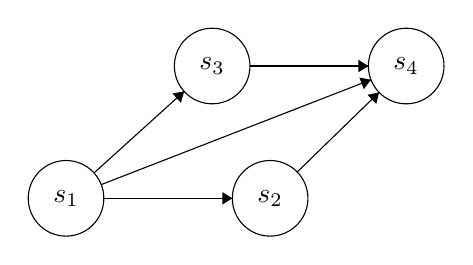
\begin{tikzpicture}[scale=0.16]
	\tikzstyle{every node}+=[inner sep=0pt]
	\draw [black] (3.4,-18) circle (3);
	\draw (3.4,-18) node {$s_1$};
	\draw [black] (19.6,-18) circle (3);
	\draw (19.6,-18) node {$s_2$};
	\draw [black] (30.4,-7.5) circle (3);
	\draw (30.4,-7.5) node {$s_4$};
	\draw [black] (15,-7.5) circle (3);
	\draw (15,-7.5) node {$s_3$};
	\draw [black] (6.4,-18) -- (16.6,-18);
	\fill [black] (16.6,-18) -- (15.8,-17.5) -- (15.8,-18.5);
	\draw [black] (21.75,-15.91) -- (28.25,-9.59);
	\fill [black] (28.25,-9.59) -- (27.33,-9.79) -- (28.02,-10.51);
	\draw [black] (5.62,-15.99) -- (12.78,-9.51);
	\fill [black] (12.78,-9.51) -- (11.85,-9.68) -- (12.52,-10.42);
	\draw [black] (18,-7.5) -- (27.4,-7.5);
	\fill [black] (27.4,-7.5) -- (26.6,-7) -- (26.6,-8);
	\draw [black] (6.2,-16.91) -- (27.6,-8.59);
	\fill [black] (27.6,-8.59) -- (26.68,-8.41) -- (27.04,-9.34);
	\end{tikzpicture}
	\vspace{0.4cm}
	\caption{The corresponding graph.}
	\label{figure:graph_example}
\end{subfigure}
\caption{An example of graph generated by Cucumber*.}
\label{figure:cucumber_flow}
\end{figure}

\subsection{Test case paths detection}

Once the parsing process of a feature file ends, the final graph is made up by nodes (scenarios) and edges (links between two scenarios). To understand how many scenarios can be generated, we need to know how many test paths there are in the graph. A test case path in a graph is a sequence of test cases (scenarios) that are executed visiting one path. Figure \ref{figure:test_case_path_example} shows an example of a test case path.

\begin{figure}[H]
	\centering
	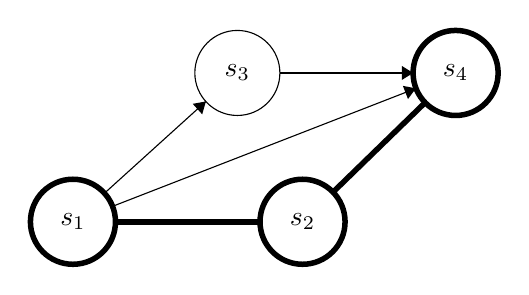
\begin{tikzpicture}[scale=0.18]
	\tikzstyle{every node}+=[inner sep=0pt]
	\draw [black, line width=0.7mm] (3.4,-18) circle (3);
	\draw (3.4,-18) node {$s_1$};
	\draw [black, line width=0.7mm] (19.6,-18) circle (3);
	\draw (19.6,-18) node {$s_2$};
	\draw [black, line width=0.7mm] (30.4,-7.5) circle (3);
	\draw (30.4,-7.5) node {$s_4$};
	\draw [black] (15,-7.5) circle (3);
	\draw (15,-7.5) node {$s_3$};
	\draw [black, line width=0.7mm] (6.4,-18) -- (16.6,-18);
	\draw [black, line width=0.7mm] (21.75,-15.91) -- (28.25,-9.59);
	\draw [black] (5.62,-15.99) -- (12.78,-9.51);
	\fill [black] (12.78,-9.51) -- (11.85,-9.68) -- (12.52,-10.42);
	\draw [black] (18,-7.5) -- (27.4,-7.5);
	\fill [black] (27.4,-7.5) -- (26.6,-7) -- (26.6,-8);
	\draw [black] (6.2,-16.91) -- (27.6,-8.59);
	\fill [black] (27.6,-8.59) -- (26.68,-8.41) -- (27.04,-9.34);
	\end{tikzpicture}
	\vspace{0.3cm}
	\caption{An example of a test case path.}
	\label{figure:test_case_path_example}
\end{figure}

The problem of finding test cases paths starting from a graph is known as a graph coverage problem. It can be solved by choosing the best \textit{test coverage criterion} that fits our needs. There are a several of criteria we can consider for our work: Node Coverage (NC), Edge Coverage (EC), Edge-Pair Coverage (EPC), Simple Round Trip Coverage (SRTC), Complete Round Trip Coverage (CRTC), Prime Path Coverage (PPC) \cite[p. 25-42]{book:introduction_to_software_testing}. These criteria can be implemented extending common algorithm such as the Breadth-first search (BFS) or the Depth-first search (DFS). Furthermore, each criterion defines test requirements (TR) in terms of properties of test paths in a graph. For instance, a typical one is met by visiting a particular node or edge.

Our TR is to cover all the possible test paths in the graph generated in the previous step. The only criterion that meets our requirement is the Complete Path Coverage (CPC). However, this method is not feasible for graphs with cycles\cite[p. 36]{book:introduction_to_software_testing}. In fact, graph with loops has an infinite number of paths, so our TR can not be satisfied.

In order to archive the goal of obtaining test case paths from the graph we use a Breadth-first search visit, assuming that the graph in input has no cycles. This is another limit we post to our prototype. However, it is necessary to solve the problem of the infeasible paths in the early phase of the development. Moreover, we plan to use the Prime Path Coverage (PPC, \cite[p. 36]{book:introduction_to_software_testing}) criterion in the near future for finding prime test paths. According to \cite{book:introduction_to_software_testing}, the advantages are:

\begin{enumerate}
\item The process is guaranteed to terminate because the length of the longest possible prime path is the number of nodes.
\item It can be computed by a simple dynamic programming algorithm.
\item The algorithm requires loops to be executed.
\end{enumerate}

The Breath-First search algorithm we implemented is shown below. We assume that there is a \textit{.last\_path()} method which gets the last subset added in the $curr$ set, and a \textit{.last\_node()} method which obtains the last node added in a set of sub paths.

\vspace{0.4cm}
\begin{algorithm}[H]
	\KwIn{A graph $G$}
	\KwIn{An initial node $n$}
	\KwOut{A list of paths $P$}
	Mark $n$ as visited\;
	Let $Q$ a queue\;
	Let $P$ be the set of final test case paths in $G$\;
	$Q$.push([$n$])\;
	$P \leftarrow \emptyset$\;

	\While{$Q$ is not empty}{
		Let $curr \leftarrow Q$.pop()\;
		Mark last node of $curr$.last\_path() as visited\;
		\If{$curr$.last\_path().adj() is empty}{
			$P$.add\_subset($curr$)\;
		}
		\ForEach {$v \in curr$.last\_path().adj()}{
			Let $tmp\_path \leftarrow curr$\;
			$tmp\_path$.insert($v$)\;
			\uIf{$v$ is not visited}{
				$Q$.push($tmp\_path$)\;
			}
			\Else{
				$P$.add\_subset($tmp\_path$)\;
			}
		}
	}
	\textbf{return} $P$\;
	\vspace{0.2cm}
	\caption{Algorithm for obtaining a list of test paths from a graph.}
\end{algorithm}
\vspace{0.4cm}

Assuming the graph in Figure \ref{figure:graph_example} and the initial node $s_1$ as inputs to the algorithm above, the result set of test case paths is the following:
\begin{center}
$P = \Set{ \Set{s_1,s_3,s_4}, \Set{s_1,s_4}, \Set{s_1,s_2,s_4} }$ \nonumber
\end{center}

\newpage
\subsection{Scenario generation}

To generate new test cases we use the set of unique paths $P$ as input. More precisely, each path will be considered as a new scenario that will be executed by Cucumber*. The crucial part of this process is to understand how new scenarios can be created for each path in $P$.

To understand how we can define a scenario that is made up by other scenarios, we consider every test case as a set of steps. For instance if we consider the scenarios in the subset $\Set{s_1,s_4}$, we can define the following sets of steps:
\begin{align}
s_1 &= \Set{Step_i, \dots, Step_n} \nonumber \\
s_4 &= \Set{Step_k, \dots, Step_m} \nonumber
\end{align}
The idea is to create a new scenario which is composed by the union of all the steps included in $s_1$ and $s_4$. As result, we obtain one single set, maintaining the order between subsets.
\begin{align}
Scenario =& \Set{Step_i, \dots, Step_n} \cup \Set{Step_k, \dots, Step_m} \nonumber \\
=& \Set{Step_i, \dots, Step_n, Step_k, \dots, Step_m} \nonumber
\end{align}
Now that we know how to compose scenarios in a single one, we have to understand how the scenario defined above can be executed by Cucumber*. The solution to this problem can be found considering the AST explained in Section 2.5. To allow Cucumber* to execute new scenarios, we need to add them as children of the root node \textit{Feature}. Moreover, the new nodes must keep the structure defined by the Table \ref{table:node_structure}. Hence, we need a keyword and a plain-text description for each composition.

The keyword problem is solved because we are adding new scenarios to the tree, so we can simply set their keywords to \textit{Scenario}. On the other side, their plain-text values are more difficult to find because each path crossed by the algorithm should have a meaningful name. The reason is that, testers should be able to recognize instantaneously which test case path is failed. A solution we found is to concatenate the names of the single scenarios cross the path using the symbol ``$\rightarrow$'' as follows:
\begin{center}
$scenario_1 \rightarrow scenario_2 \rightarrow \dots \rightarrow scenarios_n$ \nonumber
\end{center}
In our case the plain-text values will result the following:
\begin{center}
$Names = \Set{ \Set{s_1 \rightarrow s_3 \rightarrow s_4}, \Set{s_1 \rightarrow s_4}, \Set{s_1 \rightarrow s_2 \rightarrow s_4} }$
\end{center}

Once Cucumber* has the names of the new scenarios, a new node for each one is added to the AST. However, the nodes have no children, so no steps are executed for those scenarios. To add all the steps as children of the new scenarios, it is necessary to find each step node in the AST. The tree is visited and all the nodes found are cloned and added as children of the right scenario. The result of the final AST can be visible in Figure \ref{figure:ast_cucumber_with_link}.

\begin{figure}[h!]
	\centering
	\vspace{0.1cm}
	\synttree[Feature
					[Login]
					[Logout]
					[Login$\rightarrow$Logout
					[$Step_i$]
						[\dots]
						[$Step_n$]
						[$Step_k$]
						[\dots]
						[$Step_m$]
					]
				]
	\vspace{0.2cm}
	\caption{An example of an Abstract Syntax Tree built by Cucumber*.}
	\label{figure:ast_cucumber_with_link}
\end{figure}

The algorithm which adds new scenarios to the AST is written above. The input are the set of paths produced by the previous step and the AST resulted from the parsing of a feature file.

\vspace{0.4cm}
\begin{algorithm}[H]
	\KwIn{A set of paths $P$, An AST $T$}
	\KwOut{An AST $T$ which contains also generated scenarios}
	Let $r$ be the root of $T$\;
	\ForEach {$p \in P$}{
		Let $name$ be the name of the path\;
		$T$.add\_node\_to\_root(``Scenario'', $name$)\;
		\ForEach {$node \in p$}{
			Let $S$ be the set of steps in $node$\;
			\ForEach {$step \in S$}{
				$step\_node \leftarrow T$.find\_node($step$)\;
				$t$.add\_child($step\_node$)\;
			}
		}
	}
	\textbf{return} $T$\;
	\vspace{0.2cm}
	\caption{Algorithm for generating new scenarios.}
\end{algorithm}
\vspace{0.4cm}

Finally, when the AST is complete and every test case path is added to the tree, Cucumber* executes all the scenarios in the tree by visiting it. No other operations are needed and Cucumber* shows on the output all the scenarios that belong to the tree. An example output of Cucumber* can be seen in Figure \ref{figure:scenario_example_next_scenario_executed}.

As can be seen, no \textit{Next\_Scenario} definitions appear in the output. The number of executed scenarios is equal to:
\begin{center}
Number of written scenarios + $|P|$
\end{center}

\newpage
\begin{figure}[H]
\begin{minted}[fontsize=\small,frame=single]{gherkin}
Feature: Login and logout as collector

  Scenario: Login
    Given I am on the login page
    When I sign in as "collector@example.com"
    Then I should see "Available Offers"

  Scenario: Logout
    Given I am logged in as "collector@example.com"
    When I sign out
    Then I should be redirected to the login page

  Scenario: Login->Logout
    Given I am on the login page
    When I sign in as "collector@example.com"
    Then I should see "Available Offers"
    Given I am logged in as "collector@example.com"
    When I sign out
    Then I should be redirected to the login page

3 scenarios (3 passed)
12 steps (12 passed)
0m0.011s
\end{minted}
\vspace{-1em}
\caption{The result of the execution of Cucumber*.}
\label{figure:scenario_example_next_scenario_executed}
\end{figure}

\newpage
\section{Results}

Figure \ref{figure:kaboom} shows how the feature file shown in Figure \ref{figure:scenario_example_problems} can be rewritten using Gherkin* and Cucumber*.

\begin{figure}[H]
\begin{minted}[fontsize=\small,frame=single,linenos=true]{gherkin}
Feature: Example of Collectors’ actions

  Scenario: Login
    Given I am on the login page
    When I sign in as "collector@example.com"
    Then I should see "Available Offers"
  Next_Scenario: One donation
  Next_Scenario: Two donations
  Next_Scenario: Logout

  Scenario: One donation
    When I publish a new donation
    Then I should see the last donation in the list of donations
  Next_Scenario: Two donations
  Next_Scenario: Logout

  Scenario: Two donations
    When I publish two new donations
    Then I should see the last 2 donations in the list of donations
  Next_Scenario: Logout

  Scenario: Logout
    When I sign out
  Next_Scenario: Redirect

  Scenario: Redirect
    Then I should be redirected to the login page
\end{minted}
\vspace{-1em}
\caption{How a feature file can be written using Gherkin*.}
\label{figure:kaboom}
\end{figure}

We note that two scenarios have been removed because we can execute the same actions by compose scenarios that are written in this file. Moreover, to avoid step duplication, we wrote a new scenario to test the redirect to the login page. All the written scenarios focus on steps that belong to the second category. As result, no duplicate steps occur.

In this feature file there are five \textit{Scenario} and seven \textit{Next\_Scenario} definitions. Hence, the result graph shown in Figure \ref{figure:final_example} has five nodes and seven edges.

\begin{figure}[H]
	\centering
	\tiny{
	\begin{tikzpicture}[scale=0.2]
	\tikzstyle{every node}+=[inner sep=0pt]
	\draw [black] (13.9,-3.8) circle (3);
	\draw (13.9,-3.8) node {$\substack{One\\donation}$};
	\draw [black] (4.6,-13.5) circle (3);
	\draw (4.6,-13.5) node {$Login$};
	\draw [black] (30.4,-3.8) circle (3);
	\draw (30.4,-3.8) node {$\substack{Two\\donations}$};
	\draw [black] (34.8,-13.5) circle (3);
	\draw (34.8,-13.5) node {$Logout$};
	\draw [black] (45.3,-13.5) circle (3);
	\draw (45.3,-13.5) node {$Redirect$};
	\draw [black] (6.68,-11.33) -- (11.82,-5.97);
	\fill [black] (11.82,-5.97) -- (10.91,-6.2) -- (11.63,-6.89);
	\draw [black] (16.9,-3.8) -- (27.4,-3.8);
	\fill [black] (27.4,-3.8) -- (26.6,-3.3) -- (26.6,-4.3);
	\draw [black] (31.64,-6.53) -- (33.56,-10.77);
	\fill [black] (33.56,-10.77) -- (33.69,-9.83) -- (32.77,-10.25);
	\draw [black] (37.8,-13.5) -- (42.3,-13.5);
	\fill [black] (42.3,-13.5) -- (41.5,-13) -- (41.5,-14);
	\draw [black] (7.41,-12.44) -- (27.59,-4.86);
	\fill [black] (27.59,-4.86) -- (26.67,-4.67) -- (27.02,-5.61);
	\draw [black] (7.6,-13.5) -- (31.8,-13.5);
	\fill [black] (31.8,-13.5) -- (31,-13) -- (31,-14);
	\draw [black] (1.4,-9.2) -- (2.81,-11.09);
	\fill [black] (2.81,-11.09) -- (2.73,-10.15) -- (1.93,-10.75);
	\draw [black] (16.62,-5.06) -- (32.08,-12.24);
	\fill [black] (32.08,-12.24) -- (31.56,-11.45) -- (31.14,-12.35);
	\end{tikzpicture}
	}
	\caption{The graph built by Cucumber*.}
	\label{figure:final_example}
	\vspace{0.2cm}
\end{figure}

\noindent As it can be seen, in the graph there are four test case paths, so the number of scenarios executed by Cucumber* is:
\begin{align}
\text{Total} =& \text{ Number of written scenarios} + |P| \nonumber \\
=& \text{ } 5 + 4 = 9 \nonumber
\end{align}

The result output of the execution of Cucumber* for the file shown in Figure \ref{figure:kaboom} is shown in Figure \ref{figure:kaboom_output}. Consider that in the original file the number of steps in the output was equal to 20.

\begin{figure}[H]
\begin{minted}[fontsize=\small,frame=single,linenos=true]{gherkin}
9 scenarios (9 passed)
37 steps (37 passed)
0m0.063s
\end{minted}
\vspace{-1em}
\caption{The result of the execution of Cucumber*.}
\label{figure:kaboom_output}
\end{figure}
